\documentclass[10pt,a4paper]{article}
\usepackage[latin1]{inputenc}
\usepackage{amsmath}
\usepackage{amsfonts}
\usepackage{amssymb}
\usepackage{graphicx}
\title{Finite Element Method Computer Assignment 4.1.1}
\begin{document}

\begin{figure}[t]
	\centering
	
\includegraphics[width=0.5\textwidth]{TU_d_line_P1_color_1.jpg}
\end{figure}

\begin{center}
	\textbf{Computer Assignment 4.1.1}\\
	\textbf{MMP Finite Element Methods (WI4243AP-FE)}
	\begin{tabular}{lr}
		\textbf{Shaikh Bechan} & \textbf{4146425}\\
		\textbf{Zubin Ramlakhan} & \\
	\end{tabular}
\end{center}

\section{Introduction}
The following is a report containing the evaluation of the heat equation with the finite element method.
First the problem is defined followed by the derivation of the element matrix and vector.

\section{Problem formulation}
Consider a rectangular plate, with width, $b$, and height, $h$. In the center of the plate is a rectangular part, of a different material, with width, $b_0$ and height, $h_0$. $A$ denotes the outer part of the plate while $B$ denotes the inner part.

	\begin{figure}[t]
		\centering
		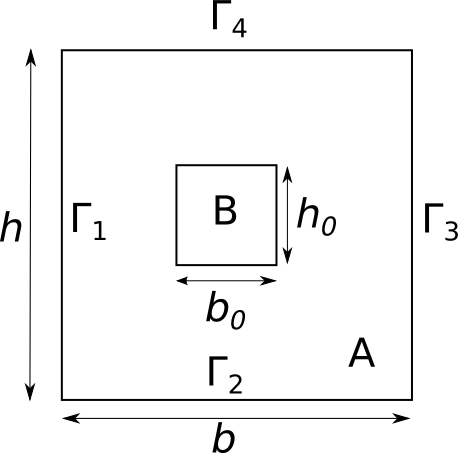
\includegraphics{schem.png}
		\caption{caption}
		\label{fig:schem}
	
	\end{figure}

Figure ~\ref{fig:schem} shows a schematic of the rectangular plate. The stationary heat equation is given by the two-dimensional equation 

\begin{equation}
	-\nabla \cdot (k \nabla T) = 0
\end{equation}

with heat conductivity $k$ and temperature $T$. The thermal conductivity is different in each material, i.e. $ k|_A = k_A $ and $k|_B = k_B $.

The boundary of $A$, $\partial A$,  is divided in four segments such that $\partial A = \Gamma_1 \cup  \Gamma_2 \cup  \Gamma_3 \cup  \Gamma_4$. On these boundaries the following conditions hold:

\begin{equation}
T|_{\Gamma_1} = T_0
\end{equation}

\begin{equation}
\nabla T|_{\Gamma_2} = T_0
\end{equation}

\begin{equation}
T|_{\Gamma_3} = T_0
\end{equation}

\begin{equation}
k\frac{\partial T}{\partial n}|_{\Gamma_4}=-\alpha(T_w - T_{\infty})
\end{equation}

In words, the temperature at boundaries $\Gamma_1$ and $\Gamma_3$ are held constant at $T=T_0$. The flux at $\Gamma_2$ is zero while $\Gamma_4$ obeys Newton's heat transfer relation with $T_{\infty}$ the environment temperature and $T_w$ the temperature at the wall.

In this problem a symmetry plane is present. This plane runs along the midsection of the plate in the vertical direction. Here, to ensure symmetry, the gradient of the temperature must be zero.

\newpage

\section{Minimization problem}
A partial differential equation can be related to an equivalent minimization problem with the following theorem:\\

\textit{Let $L$ be a linear, symmetric, positive differential operator defined of space $\Sigma$ and let}
\begin{equation}\label{eq:pde}
Lu=f
\end{equation}
\textit{Then the solution $u$ minimizes the functional}
\begin{equation}\label{eq:min}
I(u) = \int _{\Omega}\{\frac{1}{2}uLu-uf\}d\Omega
\end{equation}  \textit{over the space $\Sigma$. On the other hand, if $u$ minimizes \eqref{eq:min} then $u$ satisfies \eqref{eq:pde}} \\

Another requirement $u$ should obey is homogeneous boundary conditions, a requirement $T$ fails. Even so, this theorem can still be utilized by adapting it or by making the boundary conditions homogeneous. The latter is simpler to accomplish.
\end{document}